\documentclass[ignoreonframetext,unicode]{beamer}

\usepackage[utf8]{inputenc}
\usepackage[T1]{fontenc}
\usepackage[english,russian]{babel}
\usepackage{amsmath}
\usepackage{amsfonts}
\usepackage{amssymb}
\usepackage{graphicx,pgf}
\usepackage{multimedia}
\usepackage{multicol}
\usepackage{mathtools}
\usepackage{caption} 

\captionsetup[figure]{name=}

\usetheme{Warsaw}

\useinnertheme{circles}   %внутренняя тема
%\useoutertheme{smoothbars}   %внешняя тема
\usecolortheme{seahorse}     %цветовая схема
%\usefonttheme{serif}    %шрифты
%\defbeamertemplate*{footline}{shadow theme}
%\setbeameroption{hide notes}

\graphicspath{{./style/}{./figures/}}

%номера слайдов
\newcommand*\oldmacro{}%
\let\oldmacro\insertshorttitle%
\renewcommand*\insertshorttitle{%
	\oldmacro\hfill%
	\insertframenumber\,/\,\inserttotalframenumber}
\RequirePackage{caption}
\DeclareCaptionLabelSeparator{defffis}{ }
\captionsetup{justification=centering,labelsep=defffis}

%\title{Курсовая работа}
%\subtitle{Численные схемы для аппроксимации неограниченных решений при моделировании обтекания профиля крыла в вихревых методах}
\title[Аэроупргугая модель]{Аэроупругая модель сегментного надроторного кольца}
\author[Пиневич В.\,Г.]{Выполнил: Пиневич В.\,Г.\and\\[0.5mm] Научный руководитель: Селиванов А.\,В.}

\institute[каф. Прикладная математика ФН-2]{группа ФН2-81Б}
\date{\today}
\titlegraphic{
\includegraphics[width=2cm]{logo.png}}
%\renewcommand{\vec}[1]{\text{\mathversion{bold}${#1}$}}


\begin{document}
	
	\begin{frame}[plain]
		\maketitle
		%\insertshortinstitute{Группа ФН2-41Б}
	\end{frame}


	\begin{frame}{Практическое применение}
		\vspace*{-10mm}
		\begin{figure}[!htbp]
			\center{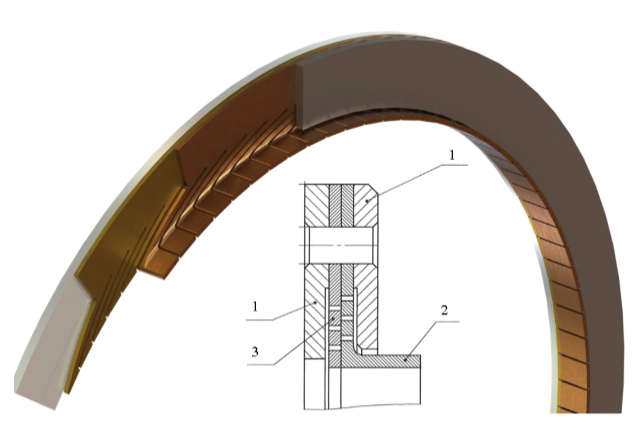
\includegraphics[width=\textwidth, height=0.6\textwidth]{vved-2.png}}
			\caption{Схема сегментного надроторного кольца (на примере пальчикового уплотнения)}
			\label{vved-2}
		\end{figure}
	\end{frame}

	\begin{frame}{Постановка задачи}
		\vspace*{2mm}
	\begin{enumerate}	
	\item Построить модель для исследования положения равновесия сегментов надроторного кольца в потоке жидкости.
	\item Исследовать устойчивость найденного положения равновесия.
\end{enumerate}
		
		\vspace*{-4mm}
	\begin{figure}[!htbp]
		\center{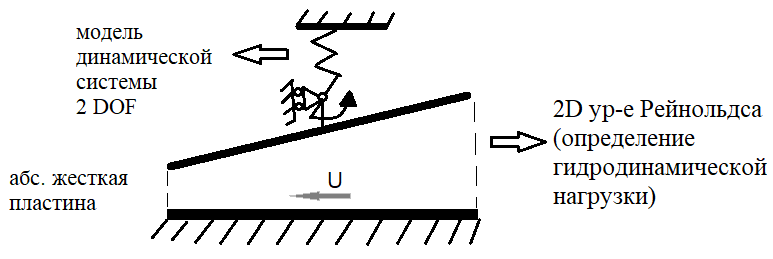
\includegraphics[width=1\textwidth, height=0.5\textheight]{pruzina-text.png}}
		\caption{Сечение модели}
		\label{pruzina}
	\end{figure}	
		
	
		
	\end{frame}

	\begin{frame}{Уравнение Рейнольдса}
		
		\begin{block}{}
			\[
			\frac{\partial}{\partial x} \left(h^3 \frac{\partial p}{\partial x} \right) + \frac{\partial}{\partial z} \left(h^{3} \frac{\partial p}{\partial z} \right) = 6 \mu U \frac{\partial h}{\partial x}
			\]
		\end{block}
		
		\vspace*{-10mm}
		\begin{columns}
	
		\column{0.5\textwidth}`
			\begin{block}{Граничные условия}
				$p(x, 0) = p_{\text{в}}$\\ 
				$p(0, z) = p(L, z) = p(x, L) = p_{\text{н}}$
			\end{block}
			\begin{block}{}
			$h = h(x, z)$ --- функция зазора \\
			$p = p(x, z)$ --- давление жидкости \\
			$\mu$ --- коэффициент вязкости \\
			$U$ --- скорость ротора
			\end{block}

	
	\column{0.5\textwidth}`
	\begin{figure}[!htbp]
	\centering
	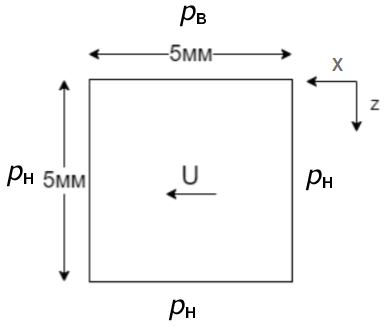
\includegraphics[width=1\textwidth, height=0.5\textheight]{taskGU}%
	\caption{Cхема расчетной области}
	\vspace*{-2mm}
	\label{ser_graph}
\end{figure}

		\end{columns}
		
		
		
	\end{frame}	

\begin{frame}{Решение уравнения Рейнольдса МКЭ}
		



	\begin{block}{Функции формы}
		\[
			\begin{cases}
				N_1 = 1 - \frac{\xi}{L} - \frac{\zeta}{H} + \frac{\xi  \zeta}{L  H}, \\
				N_2 = \frac{\xi}{L} - \frac{\xi  \zeta}{L  H}, \\
				N_3 = \frac{\xi  \zeta}{L H}, \\
				N_4 = \frac{\zeta}{H} - \frac{\xi  \zeta}{L  H} \\
			\end{cases}
			\label{form-func}
		\]
	\end{block}


\begin{block}{Аппроксимирующая функция}
	\[
	\tilde{p} = p_1 N_1 + p_2 N_2 + p_3 N_3 + p_4 N_4
	\]
\end{block}

\begin{block}{Приведение к форме Галеркина}
	\begin{equation*}
		\int_{S_i} {\left( \frac{\partial[N]^T}{\partial \xi} h^3 \frac{\partial \tilde{p}}{\partial \xi}  +  \frac{\partial[N]^T}{\partial \zeta} h^3 \frac{\partial \tilde{p}}{\partial \zeta}  - [N]^T 6 \mu U \frac{\partial h}{\partial \xi}\right) d\xi dz\zeta} = 0
	\end{equation*}
\end{block}
	
\end{frame}

\begin{frame}{Результаты расчетов}
	

	
	\begin{columns}
		
	
		\column{0.5\textwidth}
		\vspace*{-10mm}
		\begin{figure}[!htbp]
			\center{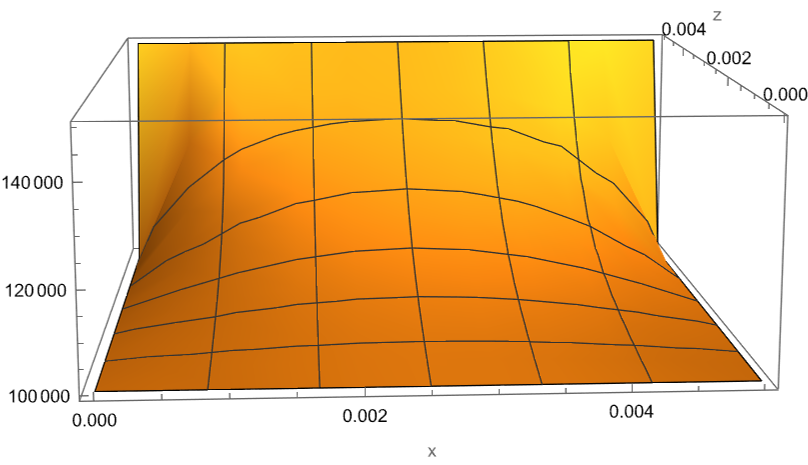
\includegraphics[width=1.13\textwidth, height=0.68\textheight]{res_static-2.png}}
			\caption{Распределение давления $h = 0.001$~м}
			\label{res_static}
		\end{figure}
	
	
	\vspace*{-7mm}
		\column{0.5\textwidth}
		\begin{figure}[!htbp]
			\center{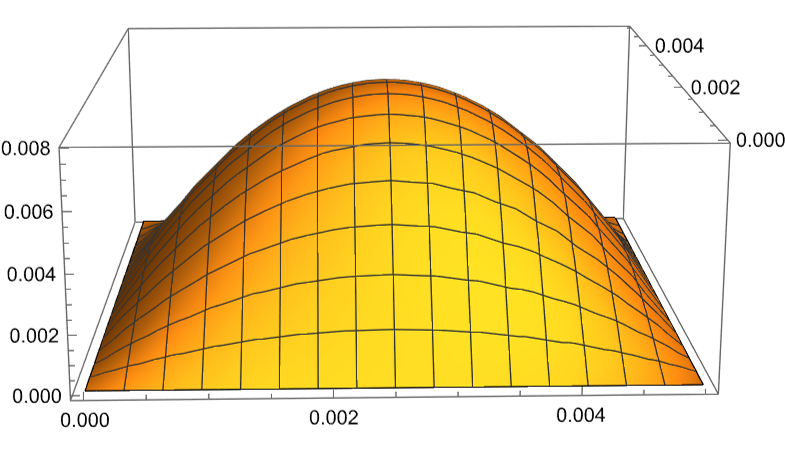
\includegraphics[width=1\textwidth, height=0.5\textheight]{check_func_1.png}}
			\caption{Проверочная функция}
			\label{check_func_1_pic}
		\end{figure}
		\vspace*{-2mm}
		\begin{block}{}
			\begin{equation*}
				\vspace*{5mm}
				{\scriptstyle 
					f(x, z) = -2 \frac{\pi x }{0.005} \sin{\left(\frac{\pi z}{0.005}\right)} \left(x - 0.005\right)
				}
			\end{equation*}
		\end{block}
		
	
		
	\end{columns}

	
\end{frame}

\begin{frame}{Верификация программы}
	\vspace*{-1mm}
	\begin{block}{Проверочная функция}
		\begin{equation*}
			f(x, z) = -2 \frac{\pi z}{0.005} \sin{\frac{2 \pi z}{0.005}} \sin{\frac{4 \pi x}{0.005}}
			\label{check_func_2}
		\end{equation*}
	\end{block}
	
	\vspace*{-6mm}
	\begin{columns}
		
		\column{0.5\textwidth}
		
		\begin{figure}[!htbp]
			\center{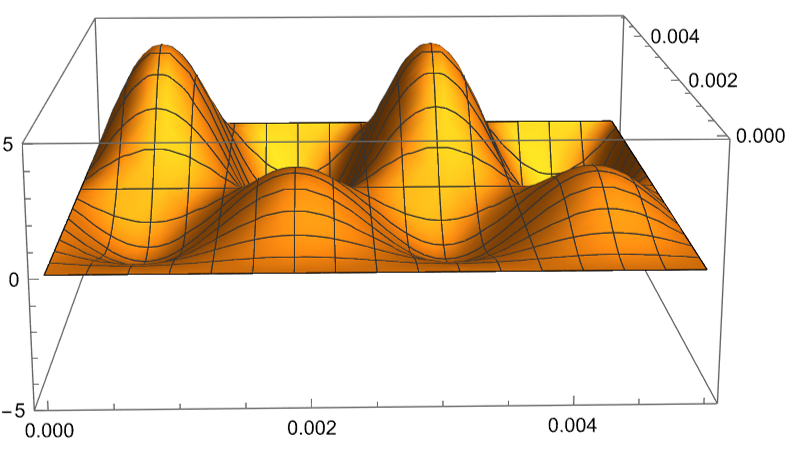
\includegraphics[width=\textwidth, height=0.35\textheight]{check_func_2.png}}
			\caption{Проверочная функция}
			\label{check_func_2_pic}
		\end{figure}
		
		\column{0.5\textwidth}
		\begin{figure}[!htbp]
			\center{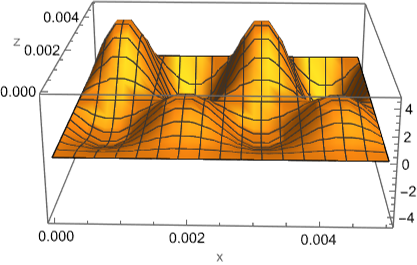
\includegraphics[width=\textwidth, height=0.35\textheight]{res_check_func_2.png}}
			\caption{Решение на сетке 20 на 20}
			\label{res_check_func_2}
		\end{figure}
		
	\end{columns}
	\vspace*{-4mm}
\begin{table}[!htbp]
	\begin{tabular}{|l|l|l|}
		\hline
		\multicolumn{1}{|c|}{Размерность сетки} & \multicolumn{1}{c|}{Разность, Па} & Погрешность, \% \\ \hline
		5 на 5                                  & 0.969                              & 21.31            \\ \hline
		10 на 10                                & 0.260                              & 5.7            \\ \hline
		20 на 20                                & 0.065                              & 1.4            \\ \hline
	\end{tabular}
\end{table}
\end{frame}

\begin{frame}{Давление в расширяющемся зазоре}
	\begin{columns}
		\column{0.5\textwidth}
		\begin{figure}[!htbp]
			\center{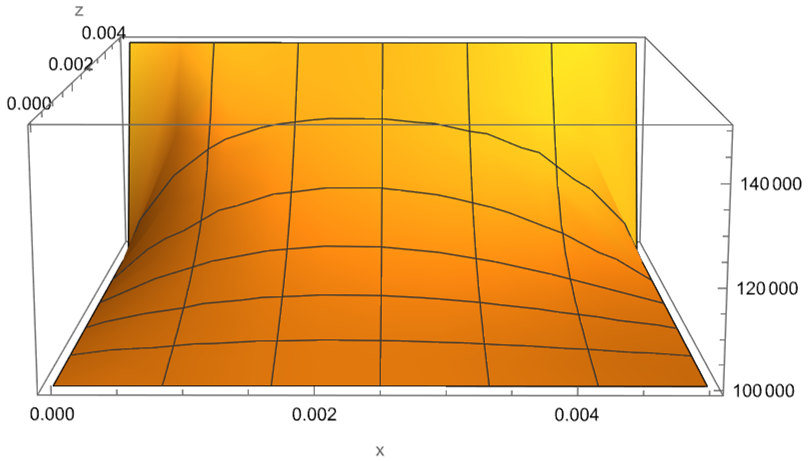
\includegraphics[width=1.1\textwidth, height=\textwidth]{res_pos-2.png}}
			\caption{Распределение давления $h = 0.15 x + 0.001$~м}
			\label{res_pos}
		\end{figure}

		
		\column{0.5\textwidth}
		\begin{figure}[!htbp]
			\center{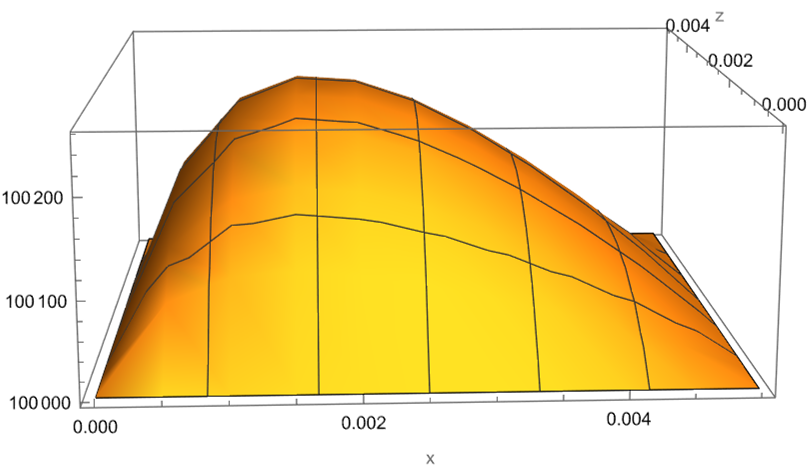
\includegraphics[width=1.1\textwidth, height=\textwidth]{zero_pos-2.png}}
			\caption{Распределение давления $h = 0.15 x + 0.001$~м, $p_{\text{в}} = p_{\text{н}}$}
			\label{zero_pos}
		\end{figure}
	\end{columns}
\end{frame}

\begin{frame}{Давление в сужающемся зазоре}	
	\begin{columns}
		\column{0.5\textwidth}
		\begin{figure}[!htbp]
		\center{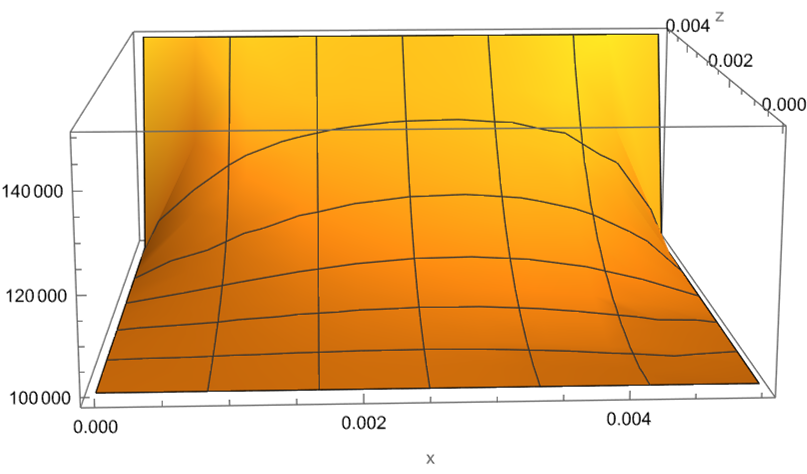
\includegraphics[width=1.2\textwidth, height=\textwidth]{res_neg-2.png}}
		\caption{Распределение давления $h = -0.15 x + 0.001$~м}
		\label{res_static}
	\end{figure}
	
	\column{0.5\textwidth}
	\begin{figure}[!htbp]
		\center{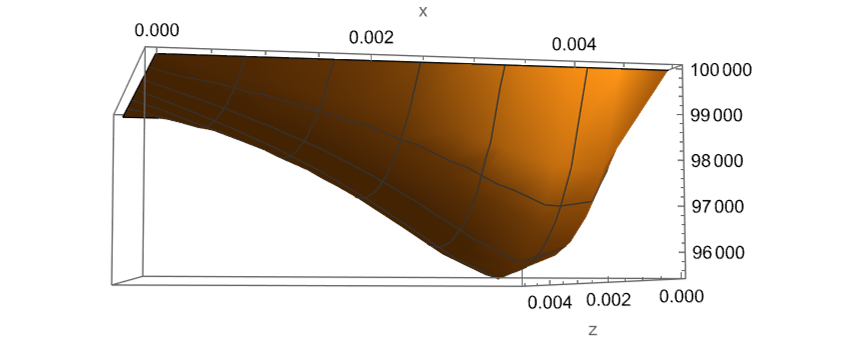
\includegraphics[width=1.2\textwidth, height=\textwidth]{zero_neg-2.png}}
		\caption{Распределение давления $h = -0.15 x + 0.001$~м, $p_{\text{в}} = p_{\text{н}}$}
		\label{zero_neg}
	\end{figure}
	\end{columns}
\end{frame}

\begin{frame}{Аэроупругая модель}
	\vspace*{-9mm}
	\begin{figure}[!htbp]
		\center{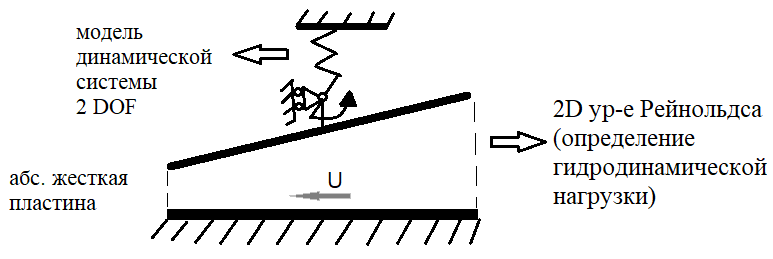
\includegraphics[width=\textwidth, height=0.48\textheight]{pruzina-text.png}}
		\caption{Сечение модели}
		\label{pruzina}
	\end{figure}	

\vspace*{-5mm}
	\begin{columns}
		\column{0.5\textwidth}
			\begin{block}{}
				\vspace*{-1mm}
			\begin{equation*}
				\begin{cases*}
					m \ddot{l} + \varepsilon \dot{l} + k l  = F \\
					J \ddot{\psi} + c \psi = M
				\end{cases*}
				\label{lagrsdfdsfsange_fin}
			\end{equation*}
		\end{block}
		\column{0.5\textwidth}
		\begin{block}{}
			\begin{equation*}
				\tilde{\tilde{p}} = p_i - p_{ext}
			\end{equation*}
		\end{block}
	\end{columns}
	
	\vspace*{-2mm}
		\begin{columns}	
			\column{0.5\textwidth}
			\begin{block}{}
				\vspace*{-4mm}
				\begin{equation*}
					\hat{p}	= N_1 \tilde{\tilde{p}}_1 + N_2 \tilde{\tilde{p}}_2 + N_3 \tilde{\tilde{p}}_3 + N_4 \tilde{\tilde{p}}_4
				\end{equation*}
			\end{block}
				\column{0.2\textwidth}
	\begin{block}{Сила}
		\vspace*{-6mm}
		\begin{equation*}{\scriptstyle 
			F_i = \int_{S_i} { \hat{p}   dx dz}
		}
		\end{equation*}
	\end{block}
	\column{0.3\textwidth}
	\begin{block}{Момент}
		\vspace*{-6mm}
		\begin{equation*}
			{\scriptstyle 
			M_i = \int_{S_i} {\hat{p}  \left(x - x_{\text{ц}} \right)  dx dz}
		}
		\end{equation*}
	\end{block}
\end{columns}


	
\end{frame}

\begin{frame}{Поиск положения равновесия}

			\begin{block}{}
			\begin{equation*}
				\begin{cases*}
					k l = F \\
					c \psi = M
				\end{cases*}
				\label{temp_ldsfsdfsdfagr}
			\end{equation*}
			\end{block}
\vspace*{-1mm}
\begin{figure}[!htbp]
	\center{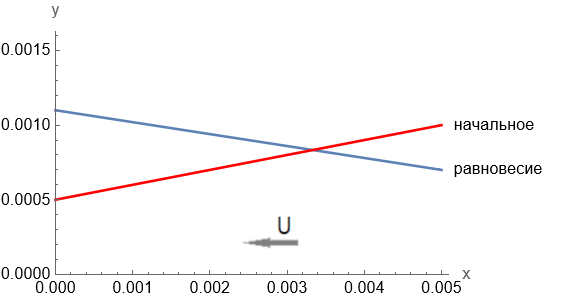
\includegraphics[width=\textwidth, height=0.5\textwidth]{part_2-zazor.png}}
	\caption{Начальное и равновесное положения}
	\label{res_chasdasdaeck_func_2}
\end{figure}



\end{frame}

\begin{frame}{Устойчивость положения равновесия}
	\vspace*{-2mm}
	\begin{columns}
		
	\column{0.5\textwidth}
	\begin{block}{}
		\vspace*{0mm}
		\begin{equation*}
			\begin{cases}
				l = l_0 + \Delta{l}, \\
				\psi = \psi_0 + \Delta{\psi}
			\end{cases}
			\begin{cases}
			\Delta{l} = \tilde{L} e^{\omega t}, \\
			\Delta{\psi} = \Psi e^{\omega t}
			\end{cases}
			\label{kjdkjsnadkjadsbafabjb}
		\end{equation*}
	\end{block}

	\column{0.5\textwidth}
	\begin{block}{}
		\vspace*{0mm}
		\begin{equation*}
			\begin{cases}
			F = F_0 + d_1 \Delta{l} + d_2 \Delta{\psi}, \\
			M = M_0 + u_1 \Delta{l} + u_2 \Delta{\psi}
			\end{cases}
			\label{kjdkjsasdsanadkjadsbafabjb}
		\end{equation*}
	\end{block}
	
	\end{columns}

\begin{block}{}
	\vspace*{-2mm}
	\begin{equation*}
		\begin{cases}
			\left( m \omega^2 - d_1 - \varepsilon \omega + k \right) \tilde{L} - d_2 \Psi = 0, \\
			- u_1 \tilde{L} + \left(J \omega^2 - u_2 + c \right) \Psi 	 = 0
		\end{cases}
		\label{kjdkjsnadkjddadsbafabjb}
	\end{equation*}
\end{block}

\vspace*{-2mm}
\begin{block}{Критерий устойчивости}
	\vspace*{-2mm}
	\begin{columns}
		
	\column{0.6\textwidth}
	\begin{equation*} 
		\begin{cases}
			a_4 = m J \\
			a_3 = - \varepsilon J \\
			a_2 = \left(c - u_2 \right) m + \left(k - d_1 \right)J \\
			a_1 = \left(u_2 - c\right) \varepsilon \\
			a_0 = d_1 \left( u_2 - c \right) - k \left( u_2 - c \right) - d_2 u_1
		\end{cases}
	\end{equation*}

	\column{0.3\textwidth}
		\begin{equation*} 
		\begin{cases}
			a_1 >  0 \\
			a_1 a_2 - a_0 a_3 > 0 \\
			\begin{vmatrix*}
				a_1 & a_0 & 0 \\
				a_3 & a_2 & a_1 \\
				0 & a_4 & a_3 
			\end{vmatrix*} > 0
		\end{cases}
	\end{equation*}
\end{columns}
\end{block}


	
\end{frame}

\begin{frame}{Заключение}
	\begin{block}{}
	\begin{enumerate}	
		\item Показано, что исследование устойчивости положения равновесия сегментов надроторного кольца в потоке жидкости можно выполнить на основе инженерного подхода, объединяющего модель Рейнольдса для течения жидкой смазки и модель колебательной системы с двумя степенями свободы.
		\item Показано возникновение подъемного гидродинамического клина в сужающемся по окружности зазоре, а также области разряжения в зазоре с расширением. Эти результаты согласуются с экспериментально наблюдаемой картиной течения в гидродинамических подшипниках и уплотнениях.
		\item Построенная математическая модель может быть использована на этапе предварительного проектирования конструкции.
	\end{enumerate}
	\end{block}	

\end{frame}	

\begin{frame}{}
	\begin{thebibliography}{00}
		\bibitem{petrov_smazka} Петров Н.П. Гидродинамическая теория смазки, М.: из-во академии наук СССР, 1948. --- 558~с.
		\bibitem{slezkin_smazka} Слезкин Н.А. Динамика вязкой несжимаемой жидкости, М.: из-во техно-теоретической литературы, 1955. --- 521~с.
		\bibitem{seligard} Селегринд Л. Примененение метода конечных элементов, М.: из-во МИР, 1979. --- 195~с.
		\bibitem{seshu} Seshu P. Textbook of
		Finite Element
		Analysis, New Dehli: PHI Learning Private Limited, 2012. --- 340~с.
		\bibitem{itmo} Григорьев А.Ю., Григорьев К.А., Малявко Д.П. Колебания
		и виброактивность элементов машин: Учеб. пособие. СПб.: Университет ИТМО, 2016. --- 136~с.
		\bibitem{sel-1}  Селиванов А.В., Дзева И.Ю., Многодисциплинарная математическая модель пальчикового уплотнения Уфа:, 2011 --- 17 c.
		\bibitem{feodosiev} Феодосьев В.И. Сопротивление материалов: Учеб. для вузов. М.: Изд-во МГТУ им.
		Н.Э. Баумана, 1999. – 592 с.
		\bibitem{nasa} Steinetz B.M., Hendricks C.R. Overview of NASA Glenn Seal Development
		Program. Nevada: NASA
		Conference Publication, 2001 --- 493 с.
		
	\end{thebibliography}
\end{frame}
\end{document} 